\documentclass{beamer}

\usepackage{txfonts}
\usepackage{hyperref}
\usepackage{fancybox}
\usepackage{xfrac}
\usepackage{cancel}

\newcommand{\heart}{\ensuremath\heartsuit}

\usepackage{mathtools,amssymb}
\newcommand{\myarrow}{\scalebox{2}[2]{$\mathclap{\curvearrowleft}\mkern2.2mu
                                                 \mathclap{\curvearrowright}$}}

\DeclareMathOperator{\Bin}{\mathrm{Bin}}

\hypersetup{colorlinks=false,linkbordercolor=red,linkcolor=green,pdfborderstyle={/S/U/W 1}}

\addtobeamertemplate{navigation symbols}{}{ \hspace{1em}    \usebeamerfont{footline}%
    \insertframenumber / \inserttotalframenumber}

\geometry{papersize={15cm,13cm}}
\usepackage{lipsum}

\makeatletter
\newenvironment<>{contdproof}[1][\proofname]{%
    \par
    \def\insertproofname{#1\@addpunct{.}}%
    \usebeamertemplate{proof begin}#2}
  {\usebeamertemplate{proof end}}
\makeatother


\setbeamertemplate{theorems}[numbered]

\newtheorem*{nonumdefinition}{Definition}
\newtheorem*{nonumproblem}{Problem}
\newtheorem*{nonumtheorem}{Theorem}
\newtheorem*{nonumremark}{Remark}
\newtheorem*{answer}{Answer}
\newtheorem*{nonumremarks}{Remarks}
\newtheorem*{nonumexamples}{Examples}
\newtheorem*{nonumsolution}{Solution}
\newtheorem*{nonumexample}{Example}
\newtheorem*{nonumproposition}{Proposition}
\newtheorem{proposition}[theorem]{Proposition}

\usepackage{tikz}
\newcommand*\mycirc[1]{%
  \tikz[baseline=(C.base)]\node[draw,circle,inner sep=.7pt](C) {#1};\:
}

\newcommand\myheading[1]{%
  \par\bigskip
  {\color{blue}{\large #1}}\par\smallskip}

%\usetheme{Warsaw}
%\usetheme{Berkeley} %sample 1

\usetheme{Berlin} % sample 2
%\usetheme{AnnArbor} % sample 3

\let\otp\titlepage
\renewcommand{\titlepage}{\otp\addtocounter{framenumber}{-1}}

\title{Lecture 11 : The Basic Numerical Quantities Associated to a Continuous $X$}
\author{}
\date{}

\begin{document}
\begin{frame}[plain]
\titlepage
\end{frame}

\begin{frame}
In this lecture we will introduce four basic numerical quantities associated to a continuous random variable $X$. You will be asked to calculate these (and the $cdf$ of $X$) given $f(x)$ on the midterms and the final.

These quantities are
\begin{enumerate}
\item The $p$-th percentile $\eta(P)$.

\item The $\alpha$-th critical value $X_{\alpha}$.

\item The expected value $E(X)$ or $\mu$.

\item The variance $V(X)$ or $\sigma^{2}$.
\end{enumerate}
I will compute all these for $\cup(a,b)$ the linear distribution and $\cup(a,b)$.
\end{frame}

\begin{frame}
\myheading{Percentiles and Critical Values of Continuous Random Variables}

\myheading{Percentiles}

Let $P$ be a number between $0$ and $1$. The $100p$-th percentile, denoted $\eta(P)$, of a continuous random variable $X$ is the unique number satisfying
\begin{equation*}
P(X\leq \eta(P))=P\tag{$\sharp$}
\end{equation*}
or
\begin{equation*}
F(\eta(P))=P\tag{$\sharp\sharp$}
\end{equation*}
So if you know $F$ you can find $\eta(P)$. Roughly
$$
\eta (P)=F^{-1}(P)
$$
\end{frame}

\begin{frame}
The geometric interpretation of $\eta(P)$ is very important

\medskip
\centerline{
\includegraphics{figure/fig1.eps}}
\smallskip

\myheading{The geometric interpretation of $(\sharp)$}

$\eta(P)$ is the number such that the vertical line $x=\eta(P)$ cuts off area $P$ to the left under the graph of $f(x)$.

(this is the picture above)
\end{frame}

\begin{frame}
\myheading{Special Case\quad The median $\widetilde{\mu}$}

The median $\widetilde{\mu}$ is the unique number so that
\begin{align*}
P(X\leq \widetilde{\mu}) &= \frac{1}{2}\\[3pt]
\text{or}\qquad F(\widetilde{\mu}) &= \frac{1}{2}
\end{align*}
so the median is the 50-th percentile.

\myheading{The picture}

\centerline{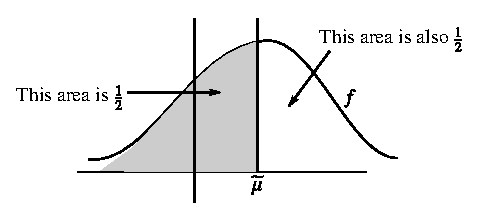
\includegraphics{figure/fig2.eps}}
\smallskip

Since the total area is 1, the area to the right of the vertical line $x=\widetilde{\mu}$ also $\dfrac{1}{2}$. So $x=\widetilde{\mu}$ bisects the area.
\end{frame}

\begin{frame}
\myheading{Critical Values}

Roughly speaking if you switch left to right in the definition of percentile you get the definition of the critical value. Critical values play a key role in the formulas for \underline{confidence intervals} (later).

\begin{nonumdefinition}
Let $\alpha$ be a real number between $0$ and $1$. Then the $\alpha$-th critical value, denoted $x_{\alpha}$, is the unique number satisfying
\begin{equation*}
P(X\geq x_{\alpha})=\alpha\tag{b}
\end{equation*}
\end{nonumdefinition}
\end{frame}

\begin{frame}
Let's rewrite (b) in terms of $F$. We have
\begin{align*}
P(X\geq x_{\alpha}) &= 1-P(X\leq x_{\alpha})\\[3pt]
                  &= 1-F(x_{\alpha})
\end{align*}
So (b) becomes
\begin{align*}
& 1-F(x_{\alpha})=\alpha\\
& F(x_{\alpha})=1-\alpha\\
& x_{\alpha} = F^{-1}(1-\alpha)\tag{bb}
\end{align*}
What about the geometric interpretation?
\end{frame}

\begin{frame}
\myheading{The geometric interpretation}

%raghu, 
\end{frame}

\begin{frame}

\end{frame}

\begin{frame}

\end{frame}

\begin{frame}

\end{frame}

\begin{frame}

\end{frame}

\begin{frame}

\end{frame}

\begin{frame}

\end{frame}

\begin{frame}

\end{frame}

\begin{frame}

\end{frame}

\begin{frame}

\end{frame}

\begin{frame}

\end{frame}

\begin{frame}

\end{frame}

\begin{frame}

\end{frame}

\begin{frame}

\end{frame}

\end{document}


